\section{Approach to Arcadia and AADL}\label{sec:app}
The workflow of our approach is shown as figure \ref{fig:wf}. Since on the one hand the Arcadia methodology and Capella modeling platform focus on high level of engineering, and on the other hand, the AADL focuses on structural modeling to describe concrete execution behaviors of components, its annex can be used to describe hybrid behaviors. Hence, in this paper, we focus on combining Arcadia and AADL model semantically using metamodels combination. To extend the semantics of Arcadia (with its profiles) and SysML to AADL, we proposed a set of operators to specify various transformation case and constitutes the transformation rules (called Transformation Rule LIB). For Transformation from Arcadia to AADL formally, we proposed a couple of metamodels of the subset of AADL and ARCADIA respectively, and their formal definitions have been given as well. As Hybrid Annex is an extension used to describe discrete and continuous behaviors, its metamodel and formal definition are also provided. For the more detailed syntax and semantics of hybrid annex, the reader is referred to \cite{Ahmad:2014:HAA:2692956.2663178}. 

Based on our defined AADL and Arcadia metamodels, system designs in Arcadia variation information can be extracted and transformed into corresponding AADL metamodels, once the new metamodels have been generated, designers can create concrete models for conducting further analysis, in this paper, we use generated AADL models to simulate the scheduling of system. The verification of the AADL model and result of the simulation are both can trace back to original Arcadia models. It can directly help designer tuning the system models, correct the vulnerabilities and flaws and improves the system performance.  


\begin{figure*}[h]
\centering
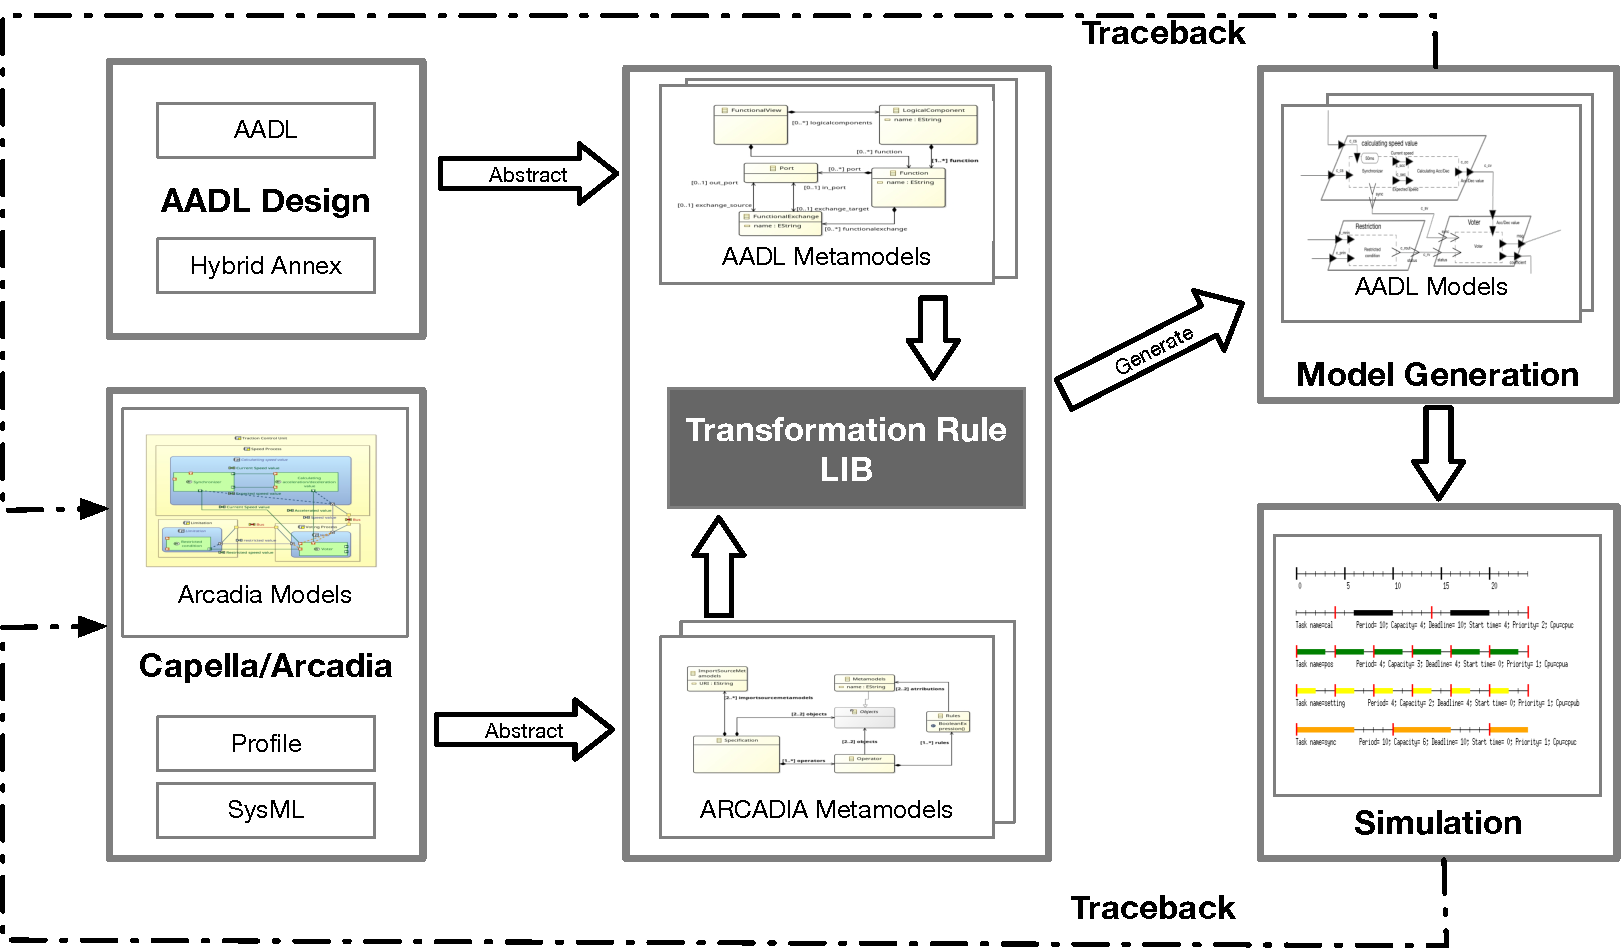
\includegraphics[width=.85\textwidth]{img/method}
\caption{Workflow}
\label{fig:wf}
\end{figure*}

\subsection{AADL and Hybrid Annex (HA)}
\subsubsection{Background of AADL}
Architecture Analysis and Design Language (AADL) is used to describe the system model, including both software and hardware (execution platform) parts. An AADL model can model the system as a hierarchy of software components bound to an execution platform and conduct a system analysis. Predefined abundant components such as thread, thread group, process, data and subprogram in soft categories, and processor, memory, device, and bus in platform categories. 

There are three kind of components in AADL:
\begin{enumerate}
\item Application software components: \textbf{data}, \textbf{subprogram}, \textbf{thread}, \textbf{thread group}, \textbf{process}, 
\item Execution platform components: \textbf{processor}, \textbf{memory}, \textbf{virtual memory}, \textbf{bus}, \textbf{virtual bus}, \textbf{device}
\item Composite component: \textbf{system}
\end{enumerate}

In AADL, each element in category of the component includes the \textit{component type and component implementation}. The type is a specification of the external interface. A component type contains features, flow specifications, property associations. A component type defines the communicational port, while component implementation specifies subcomponent and the interactive among the subcomponents. The features of AADL are designed to model the communication between different components. It is composed of \textbf{event} port, \textbf{data} port, \textbf{event data} port, parameter access, data access and bus access. Each component contains some non-functional properties.

The \textbf{thread} component includes priority, preemptive, dispatch protocol, and time-related property. And \textbf{process} component is a composition unit of \textbf{thread} component, and includes all the resource of \textbf{thread} component. The component implementation must conform to their type which includes the detail contents such as refined type, sub-components, connections, flow, functional and non-functional properties. 



\subsubsection{Software Functional Composition}
In AADL, application software components communicate each other and they rely on the processor, memory and bus of execution platform component. Even they may interactive with device components. 
\defn{(Software Functional Composition)}\label{def:sfc} A \textbf{SFC} is a seven tuples:\\ $\mathcal{A} = <Type, Impl, \Sigma_{T, I}, Port, Property, Flow,  Annex>$ \\where:
\begin{enumerate}
\item $Type$ defines the category of the components. 
\item $Impl = <Sub, Conn>$ is the corresponding specific implementation of a component type. And each implementation includes the deployment of subcomponents and connections.
\item $\Sigma_{T, I}\subset Type\times Impl$ defines the relationship of component type and component implementation.
\item $Port$ is a set of communication unit among threads. Port includes \textbf{data} port, \textbf{event} port and \textbf{data event} port. And, port is divided into \textbf{in} port, \textbf{out} port, \textbf{in out} port.
\item $Property$ is a set of non-functional feature.
\item $Flow$ specifies \textbf{flow source}, \textbf{flow sink} and \textbf{end to end flow}. 
\item $Annex$ is a set of the extensions of AADL.
\end{enumerate} %\qed


\subsubsection{Execution Platform}
AADL component model is an abstract of actual systems. So, all the application software components finally run on execution platform component and the connections between application software component are bound to \textbf{bus} component.  
\defn{(Execution Platform)} A \textbf{EP} component is defined as a six tuples:\\ $\mathcal{E} = <Type, Impl, \Sigma_{T, I}, BusAccess, Property, Annex>$ \\where: 
\begin{enumerate}
\item $BusAccess$ defines the interactive approach between \textbf{bus} component and other execution platform components.
\item $Property$ is a set of non-functional feature.
\item $Type$ defines the category of the components. 
\item $Impl$ is the corresponding specific implementation of a thread type.
\item $\Sigma_{T, I}\subset Type\times Impl$ defines the relationship of component type and component implementation.
\item $Annex$ is a set of the extensions of AADL.
\end{enumerate} %\qed

\subsubsection{Binding}
In AADL, the pre-defined property set includes \emph{deployment\_properties}, which is used to describe the deployment relationship from the software component to execution platform component. Here, we define $\emph{bind}$ as an operator between application software components and execution platform components. 
\defn{(Binding)} In the system with multiple processors, \emph{bind} is a tuple: $\mathcal{B} = <SFC, EP, \Sigma B_{S,E}>$, where
\begin{enumerate}
\item $SFC$ is a set of application software components.
\item $EP$ is a set of hardware components.
\item $\Sigma B_{S,E}$ is holistic binding relation space between software components and hardware components.
\end{enumerate} %\qed



Multiple application software components can execute on the same \textbf{processor} component or \textbf{memory}, and multiple connections between application software components can be bound to the same \textbf{bus} component. 
However, at the same time, the execution platform has limited resources, it can only support software components with restricted rules. Over many request resources lead to conflicts.

\subsubsection{Hybrid Annex}
Hybrid Annex (HA) is a lightweight extension in order to model those physical, real-world elements, or processes. HA subclauses annotate either AADL device component implementations to model the continuous behavior of sensors and actuators, or abstract component implementations to model the continuous behavior of physical processes. Ehsan Ahmad et al. proposed an HA specification consist of six sections: \textit{Assert, Invariant, Variables, Constants, Channels, and Behavior}~\cite{Ahmad:2014:HAA:2692956.2663178}. \textit{Assert} is used to declaring predicates which may be used with invariants to define a condition of operation. We use the HA to declare both discrete and continuous variables in the \textit{Variables} section, and the initial values of constants are given in \textit{constant} section. The \textit{behavior} section is used to specify the continuous behavior of the annotated AADL component in terms of concurrently-executing processes, and use continuous evolution --- a differential expression to specify the behavior of a physical controlled variable of a hybrid system. The communication between computing units and physical components are an essential part of a hybrid system, Communication between physical processes uses the channels declared in the channels section, and communicate with an AADL component relies on ports that are declared in the component's type. Continuous process evolution may be terminated after a specific time or on a communication event. There are invoked through timed and communication interrupts, respectively. A timed interrupt preempts continuous evolution after a given amount of time. A communication interrupt preempts continuous evolution whenever communication takes places along any one of the named ports or channels. The definition \ref{def:ha} gives a metamodel of Hybrid Annex which does not exist in SysML,  

\defn{(Hybrid Annex)}
    \label{def:ha}
    A \textit{Hybrid Annex} is a 8-tuple $<Ass, Ivar, Var_{hd}, Cons_{hd}, P_{roc}, ChP, Itr, B_{itr}>$, where 
\begin{enumerate}
    \item $Ass$ is a finite set of assert for declaring predicates applicable to the intended continuous behavior of the annotated AADL component.
    \item $Ivar$ is associated with assert to define a condition of operation that must be true during the lifetime.
    \item $Var_{hd}$ is a finite set of discrete and continuous variables.
    \item $Cons_{hd}$ is a finite set of constants which must be initiated at declaration.
    \item $P_{roc}$ is a finite set of processes that are used to specify continuous behaviors of AADL components.
    \item $ChP$ is a finite set of channels and ports for synchronizing processes. 
    \item $Itr$ is a finite set of time or communication interrupts.
    \item $B_{itr}: Itr \rightarrow P_{roc}$ binds interrupts to related processes.
\end{enumerate} %\qed
     

\subsection{Arcadia and SysML}
In practice, the operational added value of the MBSE approach is based on many other criteria such as the definition of project modeling objectives, the implementation of adapted methods, the skills of the teams, the involvement of the hierarchy, the integration with the existing information system and third-party tools. In short, there are other aspects to consider when evaluating when to use a SysML tool or Capella than just the language.
Arcadia presents a methodology to define, design, analyze and validate systems with software and hardware architecture. It provides a hierarchical structure with logical/functional components, physical components. Logical components deploy into physical components. Here, we define $allocate$ as an operator to describe the relationship of functional components with physical components. Formally, an $allocate$ operator is defined as a tuple: $<C_{logi}, C_{Phy}>$


\subsubsection{Logical components}
Blocks are modular units of system descriptions in SysML and are generalizations of the UML class concept. In the Arcadia, Functional chains diagrams consist of a set of SysML blocks and its interactions, named \textit{Logical components}; The notion of Logical components in Arcadia enables better expression of system engineering semantics compared to SysML, and particularly, reduces the bias towards software. SysML block definition diagrams (BDDs) and internal block diagrams (IBDs) are assigned to different abstract and refined layers, respectively. The definition of a block in SysML can be further detailed by specifying its parts; ports, specifying its interaction points; and connectors, specifying the connections among its parts and ports. This information can also be visualized using logical components in Arcadia. In the definition \ref{def:lc}, we present a metamodel of an instance of logical components.

\defn{(Logical Component)}\label{def:lc}
    A logical component chain is 8 tuples, $< C_{omp}, FPC, P_{alloc}, Ex_{comp}, F_{un}, P_{ort}, Ex_{fun}, M_{cf}>$ where,
\begin{enumerate}
\item $C_{omp}=\{\bigcup_{F_{un}}\}$ is a logical component container which contains a set of functional blocks.
\item $FPC=\{\bigcup_{P_{port}}\}$ is a functional port container which contains a set of functional ports.
\item $P_{alloc}=\{FPC, PP\}: \Sigma FPC \rightarrow PP$ donates a finite set of allocated port which represents the allocable relationship between functional port container(FPC) and physical port (PP). In Arcadia, the source functional port container is named \textit{Allocated function ports}, and the target physical port is named \textit{Allocating physical ports}.
\item $Ex_{comp} \subseteq P_{alloc} \times P_{alloc}$ is a finite set of exchange between logical components.   
\item $F_{un}$ is a finite set of functional block include their name and id attributes.
\item $P_{ort}$ is a finite set of functional ports including directions and allocation attributes.
\item $Ex_{fun} \subseteq P_{ort} \times P_{ort}$ donates a finite set of functional exchange (connection) between two functional ports, it must be pair, one is source, another is target. 
\item $M_{cf}$ : $\Sigma F_{un} \rightarrow C_{omp}$ allocate functions to a logical component container.
\end{enumerate} %\qed


\subsubsection{Physical components}
The blocks can also represent hardware component in SysML, but in the Arcadia, there are the specific notation for physical components and its port, interaction so-called Physical link. 

\defn{(Physical Component)}\label{def:pc}
    A logical component chain is 3 tuples, $< N_{ode}, PP, Ex_{fpp}, PL>$ where,
\begin{enumerate}
\item $N_{ode}$ is a execution platform, named \textit{node} in Arcadia, it could be different type of physical component (e.g, processor, board). 
\item $PP$ is the physical component port.
\item $Ex_{fpp} \subseteq P_{alloc} \times PP$ is a finite set of exchange between functiotnal allocation port and physical ports. 
\item $PL$ is physical link, it could be assigned a concrete type such as \textit{bus}.  
\end{enumerate}  %\qed


\begin{figure}[hbt]
\centering
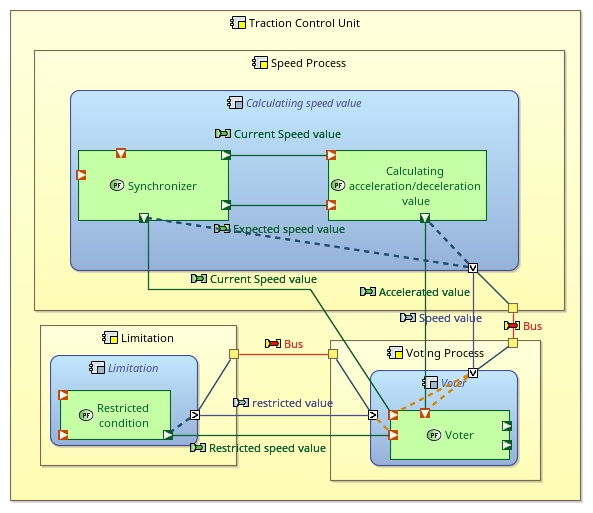
\includegraphics[width=\linewidth]{img/VTCSystem}
\caption{An example of instantiate model of kernel unit of train traction control system in ARCADIA}
\label{fig:VTCS}
\end{figure}



In the figure \ref{fig:VTCS}, there is an instance model of kernel unit of train traction control system in Arcadia as an example. We can see the yellow parts are the physical node ($N_{ode}$) and the red line is the physical link ($PL$) which connects to two physical ports ($PP$) named bus in this case. A rectangle in blue is the logical component ($C_{omp}$) which contains the functional components (the rectangle in green $F_{un}$). The deep green square with the white triangle is the outgoing port ($P_{ort}$), which connects to an incoming port ($P_{ort}$) that is drawn as a red square with white triangle and the green line is the functional exchange between two functional ports ($Ex_{fun}$). A white square with a black arrow at the edge of the logical component is the allocated port, and the dotted line in green is the allocatable relation ($P_{alloc}$) which represents the allocation between functional port containers and physical ports, and the black line is the exchange link ($Ex_{comp}$) between two port allocations.
